
% Sage Linear Algebra Quick Reference
% (c) 2013 by Barry Balof
% Licensed with the GNU Free Documentation License (GFDL)
%   http://www.gnu.org/copyleft/fdl.html
%
%  History
%
%    2009-05-10  Initial version based on Sage 3.4
%    2009-05-13  Added right paren to vector u in "vector operations" section
%    2010-08-15  Miscellaneous edits
%    2011-12-12  Update to Sage 4.8
%
%
\documentclass{article}
\usepackage{graphicx}  
\usepackage[landscape]{geometry}
\usepackage[pdftex]{color}
\usepackage{url}
\usepackage{multicol}
\usepackage{amsmath}
\usepackage{amsfonts}
\newcommand{\ex}{\color{blue}}
\newcommand{\warn}{\bf\color{red}}
\pagestyle{empty}
\advance\topmargin-.9in
\advance\textheight2in
\advance\textwidth3.0in
\advance\oddsidemargin-1.45in
\advance\evensidemargin-1.45in
\parindent0pt
\parskip2pt
% Section break, dictates column widths?
\newcommand{\hr}{\centerline{\rule{3.5in}{1pt}}}
% Adjust gap to affect spacing, page count
\newcommand{\sect}[1]{\hr\par\vspace*{2pt}\textbf{#1}\par}
% Mandatory indentation on subsidiary lines
\newcommand{\skipin}{\hspace*{12pt}}
\begin{document}
\begin{multicols*}{3}
\begin{center}
\textbf{Sage Quick Reference:\\  Combinatorics and Graph Theory}\\
Barry Balof\\
Sage Version 5.9\\
\url{http://wiki.sagemath.org/quickref}\\
GNU Free Document License, extend for your own use\\
Based on work by Rob Beezer, Steven R. Turner 
\end{center}
% backup over center environment gap
\vspace{-2ex}

%*********************************************
\sect{Lists}

{\ex\verb!L = [2,17,3,17]!}\quad an ordered list

{\ex\verb!L[i]!}\quad the $i$th element of L\\
\skipin  {\warn lists begin with the 0th element}

{\ex\verb!L.append(x)!}\quad adds $x$ to L

{\ex\verb!L.remove(x)!}\quad removes $x$ from L

{\ex\verb!L[i:j]!}\quad the $i$-th through $(j-1)$-th element of L

{\ex\verb!range(a)!}\quad list of integers from $0$ to $a-1$ \\
{\ex\verb!range(a,b)!}\quad list of integers from $a$ to $b-1$\\
{\ex\verb![a..b]!}\quad list of integers from $a$ to $b$\\
{\ex\verb!range(a,b,c)!}\\
\skipin 
every $c$-th integer starting at $a$ and less than $b$

{\ex\verb!len(L)!}\quad length of L

{\ex\verb!M = [i^2 for i in range(13)]!}\\
\skipin list of squares of integers $0$ through $12$

{\ex\verb!N = [i^2 for i in range(13) if is_prime(i)]!}\\
\skipin list of squares of prime integers between $0$ and $12$

{\ex\verb!M + N!}\quad the concatenation of lists M and N

{\ex\verb!sorted(L)!}\quad a sorted version of L (L is not changed)\\
 {\ex\verb!L.sort()!}\quad sorts  L (L is changed)

{\ex\verb!set(L)!}\quad an unordered list of unique elements

%\columnbreak
%*********************************************





%*********************************************
\sect{Permutations and Combinations}



{\ex\verb!Permutations(L)!}  list of permutations of L\\
{\ex\verb!Permutations(L,2)!}  list of 2-permutations of L\\
{\ex\verb!Combinations(L)!}  list of all combinations of L (the power set) as lists\\
{\ex\verb!Combinations(L,2)!}  list of 2-combinations of L as lists\\
{\ex\verb!Partitions(n)!}  list of unordered partitions of $n$\\
{\ex\verb!Compositions(n)!}  list of compositions (ordered partitions) of $n$\\
{\ex\verb!Subsets(n)!} list of subsets of $\{1,2,\dots n\}$ as sets.
{\ex\verb!Subsets(n,k)!} list of $k$-element subsets of $\{1,2,\dots n\}$ as sets.




\columnbreak
%*********************************************
\sect{Poset Examples Operations}
{\ex\verb!P = posets.BooleanLattice(n)!}  P is the poset of subsets of a five element set\\
{\ex\verb!P = posets.ChainPoset(6)!}  P is a 6 element chain (linear) poset\\
{\ex\verb!P = posets.AntichainPoset(6)!}  P is a 6 element chain (linear) poset\\
{\ex\verb!P = posets.DiamondPoset(8)!} P is an antichain of 6 elements, each element of which is greater than a minimal element and less than a maximal element.  \\

{\ex\verb!P = Poset({0:[3],1:[2,3],2:[3,4],3:[4],4:[]!})  Creates a poset where each element is followed by its list of successors (where transitivity is implied).  
{\ex\verb!P = Poset({0:[3],1:[2,3],2:[3,4],3:[4],4:[]!})  Creates a poset where each element is followed by its list of successors (where transitivity is implied).  




{\ex\verb!P.maximal_chains()!} List of maximal chains of P\\
{\ex\verb!P.antichains()!} List of antichains of P\\
{\ex\verb!P.linear_extensions()!} List of linear extensions of P\\


%*********************************************
\sect{Binomial and Polynomial Constructions}

{\ex\verb!binomial(a,b)!}  $\binom{a}{b}$\\
{\ex\verb!list(binomial(8, i) for i in xrange(9))!}  list of biniomial coefficients  of the form $\binom{8}{i}$ (the 8th row of Pascal's Triangle) \\
{\ex\verb!multinomial(a,b,c,d)!}  $\binom{a+b+c+d}{a,b,c,d}$


{\ex\verb!p=!} an expanded polynomial in any number of variables\\
{\ex\verb!p.coefficients()!} returns a list of the coefficients of p.  \\
{\ex\verb!p.coefficient(x^2)!} returns the coefficient of $x^2$ in p. \\ 

%*********************************************

\sect{Special Number Sequences}

{\ex\verb! fibonacci(n)!}  returns the $n$th Fibonacci Number, with $F_1=F_2=1$ \\
{\ex\verb! bell_number(n)!} returns the $n$th Bell Number\\
{\ex\verb! catalan_number(n)!}  returns the $n$th Catalan Number\\
{\ex\verb! stirling_number1(n,k)!}  $\left[{n \atop k}\right] $, the Stirling number of the first kind \\
{\ex\verb! stirling_number2(n,k)!}  $\left\{{n \atop k}\right\} $, the Stirling number of the second kind \\
{\ex\verb! a=sloane.A000045!} sets a as sequence A000045 in Sloane's OEIS.  Use {\ex\verb! sloane.A <tab>!} for a list of SAGE enabled sequences.  \\





%*********************************************
\columnbreak

\sect{Graph Constructions}
Sage has many, many (many!) examples of graphs.  Type {\ex\verb!graphs.!} then press $\langle tab \rangle$ for a complete list.  \\

{\ex\verb!G.show()!} draws a plot of G.  \\
{\ex\verb!G.plot()!} draws a plot of G.  \\
{\ex\verb!G = Graph([(1,3),(3,8),(5,2)])!}  creates a graph with specified edges (vertices are implied) \\
{\ex\verb!G = Graph({0:[1,2,3], 2:[4]})!}  creates a graph with listed adjacencies \\
{\ex\verb!G = graphs.RandomGNP(n, p)!}  creates a random graph on $n$ vertices, where each edge is included with probability $p$.  

{\ex\verb!G.add_vertex(v)!}  adds a vertex v to G.  \\
{\ex\verb!G.add_edge((a,b))!}  adds an edge (a,b) to G. \\ 
{\ex\verb!G.add_cycle([5,6,7,8])!}  adds a cycle on vertices G  (note: SAGE will use existing vertices if these are included, or add vertices as necessary.)  \\
{\ex\verb!G.delete_vertex(v)!}  deletes the vertex v from G.\\  
etc....\\

%*********************************************
\sect{Graph Queries}
{\ex\verb!G.is_planar()!}  returns True if G is planar\\
{\ex\verb!G.is_bipartite()!} returns True if G is bipartite\\  
{\ex\verb!G.is_eulerian()!} returns True if G is Eulerian\\
{\ex\verb!G.is_hamiltonian()!} returns True if G is Hamiltonian\\  
{\ex\verb!G.is_connected()!} returns True if G is connected  \\
{\ex\verb!G.is_isomorphic(H)!} returns True if G and H are isomorphic \\



%**********************************************
\sect{Graph Statistics}

{\ex\verb!G.size()!}  number of edges of G \\
{\ex\verb!G.order()!}  number of vertices of G \\ 
{\ex\verb!G.girth()!}  length of the shortext cycle of G \\ 
{\ex\verb!G.chromatic_polynomial()!} returns the chromatic polynomial of G \\
{\ex\verb!G.automorphism_group(G)!} returns the autmorphism group of G \\



\columnbreak



\sect{Graph Examples}


\begin{center}

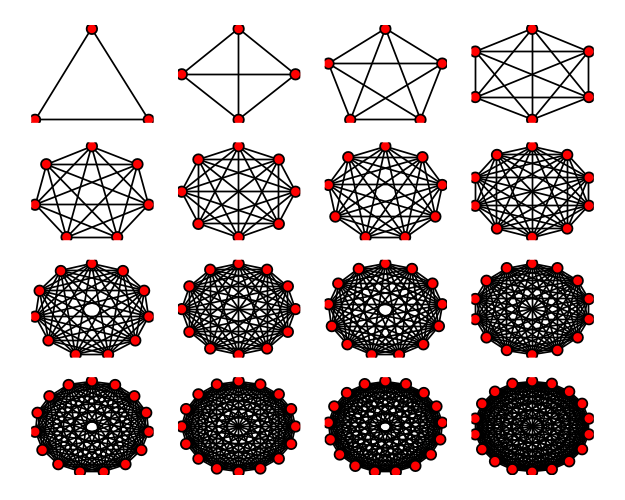
\includegraphics[scale=.4]{sage0.png} \\

$K_5$  \\

\includegraphics[scale=.4]{sage1.png} \\

Petersen Graph  \\

\includegraphics[scale=.4]{sage2.png} \\

Ladder Graph (5)  \\

\end{center}

\columnbreak

\begin{center}

\includegraphics[scale=.5]{sage3.png}\\

Cube Graph (4).  \\
Note that the vertices are labled with 0-1 strings.  \\

\end{center}


\sect{More Help}
``tab-completion'' on partial commands\\
``tab-completion'' on{\ex\verb!  <object.>!} for all relevant methods\\
{\ex\verb!<command>?!} for summary and examples\\


\end{multicols*}

\end{document}